\chapter{Planning \& Economical Analysis}\label{chap:planning}

\section{Planning}
The project development phase was divided in ``milestones'', each one trying to deliver a sort of ``functional'' product (even if in a very bare state). These were the milestones defined:
\begin{itemize}
	\item \emph{0.0 Initial proof-of-concept}: initial research, including writing a minimal input event handler kernel module capable of filtering device source events and subsitute them by ``fake'' ones.
	\item \emph{0.1 Basic kernel module}: in this phase, the very bare kernel module created in previous milestone was refactored, in order to actually be able of mapping arbitrary buttons on the device to simple keyboard key press \& release events. Initial programming API was also included here.
	\item \emph{0.2 User space tools}: started implementation of the C/C++ warapper library, plus the userspace binaries to manipulate the kernel module and load profiles into it.
	\item \emph{0.3 Mode support}: added support for mode hierarchy, both in kernel module and in C/C++ library.
	\item \emph{0.4 Axis mapping}: added support for axis mapping through bands. 
	\item \emph{0.5 Macros}: added support for ``macro'' actions.
	\item \emph{0.6 Mouse events}: added support for mouse actions, including simulating mouse movement.
	\item \emph{1.0 Initial release}: final polishing, including testing, bugfixing, and writing wiki-based user manual.
\end{itemize}

Table \ref{fig:gantt_diagram} shows the project scheduling, according to the main milestones defined, and their associated Gantt diagram (dates shown are aproximative).

The whole development of the project has entirely been made only over spare time, in order to render it compatible with my current full-time job.

\begin{figure}[tp]
\centering
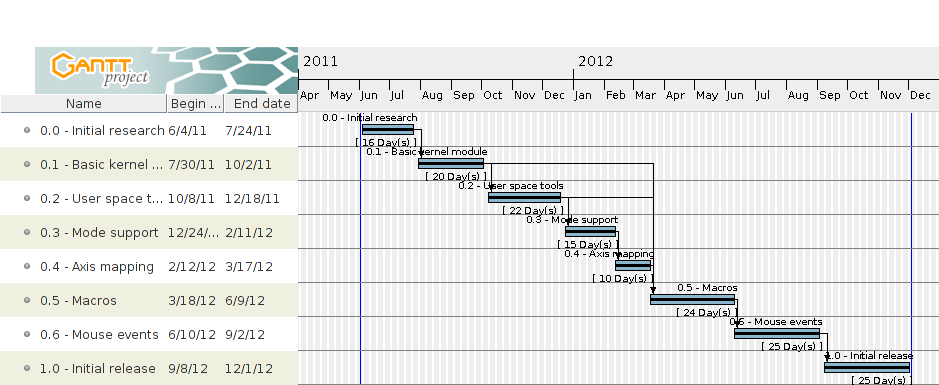
\includegraphics[width=1.6\textwidth, angle=90]{gantt}
\caption{Gantt diagram}
\label{fig:gantt_diagram}
\end{figure}


\section{Economical analysis}

The whole cost analysis is detailed in table \ref{fig:cost_analysis}.
\begin{figure}[htb]
\centering
\includegraphics[width=1.2\textwidth]{costs}
\caption{Cost analysis}
\label{fig:cost_analysis}
\end{figure}

The project has been developed using exclusively FOSS (Free and Open Source Software) tools, thus it didn't require spending any money on software licenses. Because of that, the cost of this project relies solely on the ``hardware'' part (computers and testing devices used), plus the cost of the development time, assuming a reasonable cost per hour.

The resulting software product is licensed using the GPLv2 license, and final users will be able to make use of it completely free of charge.
